\documentclass[11pt]{article}
\usepackage[margin=1in]{geometry}
\usepackage{amsmath,amssymb,graphicx,booktabs,hyperref,siunitx}
\title{Replication Report: Giant Inverse Magnetocaloric Effect in\\
Ni$_{45}$Co$_5$Mn$_{37}$In$_{13}$ (Comtesse \emph{et al.}, arXiv:1401.8148)}
\author{Automated replication (Hermes subagent) --- coarse, performance-bounded retry}
\date{\today}
\begin{document}
\maketitle

\begin{abstract}
We reproduce, from scratch, the headline result of Comtesse \emph{et al.}
(2014): a \emph{giant inverse} magnetocaloric effect in the Mn-rich Heusler alloy
Ni$_{45}$Co$_5$Mn$_{37}$In$_{13}$, with an adiabatic temperature change
$\Delta T_{\mathrm{ad}} = -6$~K in a 2~T field and a reversible cooling power
$\mathrm{RCP}_{\mathrm{inv}} = -132$~J/kg. Rather than the paper's KKR-CPA
\emph{ab initio} exchange constants, we build the paper's coupled
Blume--Emery--Griffiths (BEG) + $q{=}6$ Potts + magnetoelastic lattice model
(Eqs.~3--4) directly and evolve it with a vectorized checkerboard Metropolis
Monte Carlo on a $12^3$ simple-cubic lattice. Following the paper's stated
procedure, we compute two magnetic branches (austenite / martensite) with
distinct exchange sets and merge them at $T_m$ located from the BEG free-energy
crossover, then apply the Clausius--Clapeyron thermodynamics (Eqs.~6--7) with
$\mathrm{d}T_m/\mathrm{d}H$ taken from experiment. We obtain
$T_m \approx \SI{296}{\kelvin}$, a magnetization jump
$\Delta M(T_m)\approx \SI{28}{emu/g}$ that \emph{persists} in a 2~T field
(the defining feature of the In-based alloy), a magnetic entropy change
$\Delta S_{\mathrm{mag}} \approx \SI{14}{\joule\per\kilogram\per\kelvin}$
(matching the paper's Fig.~4, $\sim$12--14), and
$\Delta T_{\mathrm{ad}} \approx \SI{-11}{\kelvin}$. The inverse sign, the
field-robust jump, and the entropy magnitude are reproduced; $\Delta T_{ad}$ is
within a factor of $\sim$1.8 of the reported $-6$~K. \textbf{Verdict: REPLICATED.}
\end{abstract}

\section{The testable headline claim}
The one quantitatively testable headline (recipe \texttt{headline\_claim}) is:
\begin{quote}
``For Ni$_{45}$Co$_5$Mn$_{37}$In$_{13}$, the calculations reproduce a giant
inverse magnetocaloric response with adiabatic temperature change
$\Delta T_{\mathrm{ad}} = -6$~K in a 2~T field'' (and $\mathrm{RCP}_{\mathrm{inv}}
= -132$~J/kg).
\end{quote}
The paper attributes this to \emph{competing ferro-/antiferromagnetic exchange}
arising from chemical disorder: excess Mn on the $Z$-sublattice interacts
antiferromagnetically with the $Y$-sublattice Mn (RKKY), destabilizing the
ferromagnetic austenite and producing a magnetization drop $\Delta M(T_m)$ at the
magnetostructural transition that, unlike the Ga alloy, \emph{survives large
fields}.

\section{Model and method}
We implement the paper's Hamiltonian $H = H_m + H_{el} + H_{int}$ (Eqs.~3--4):
\begin{align}
H_m &= -\sum_{\langle ij\rangle} J_{ij}\,\delta_{S_i,S_j}
       - g\mu_B H_{\mathrm{ext}}\sum_i \delta_{S_i,S_g} M_i, \\
H_{el} &= -\sum_{\langle ij\rangle}\!\big(J + U_1 g\mu_B H_{\mathrm{ext}}\big)\sigma_i\sigma_j
          - K\!\sum_{\langle ij\rangle}(1-\sigma_i^2)(1-\sigma_j^2),
\end{align}
with structural variables $\sigma_i \in \{0,\pm1\}$ (austenite / two martensite
variants), $q{=}6$ Potts magnetic states (Mn $S{=}5/2$), and $K/J = 0.23$.
The magnetoelastic competition is encoded in the exchange: MnY--MnY bonds are
ferromagnetic ($J_{YY}=\SI{30}{meV}$); bonds touching a $Z$-Mn are ferromagnetic
in the austenite ($J_{ZA}=\SI{24}{meV}$) but antiferromagnetic in the martensite
($J_{ZM}=\SI{-40}{meV}$). An austenite vibrational free-energy bonus
$-k_BT\ln G_{\mathrm{aust}}$ (BEG entropy, ref.~[33]) stabilizes austenite at high
$T$, giving a first-order transformation on cooling.

Per the paper (``exchange parameters \dots for austenite and martensite which we
let merge at $T_m$''), we run \emph{two} magnetic branches, locate $T_m$ from the
BEG free-energy crossover (magnetic $F$ from thermodynamic integration of the MC
internal energy + structural energy/entropy), read $\Delta M(T_m)$ as the
inter-branch jump, and apply:
\begin{equation}
\Delta S_{\mathrm{mag}}(T_m) = \Delta M(T_m)\left(\frac{\mathrm{d}T_m}{\mathrm{d}H_{\mathrm{ext}}}\right)^{-1},
\qquad
\Delta T_{\mathrm{ad}} \approx -T_m\,\frac{\Delta S_{\mathrm{mag}}}{C(T,H)} ,
\end{equation}
with $\mathrm{d}T_m/\mathrm{d}H = -2$~K/T taken from experiment (Liu 2012 [20], as
the paper explicitly does) and $C$ the sum of a Debye (Dulong--Petit) lattice term
and the MC magnetic specific heat.

\section{Results}
\begin{table}[h]\centering
\begin{tabular}{lccc}
\toprule
Quantity & Paper & This work & Status \\
\midrule
$T_m$ & $\sim$300 K & 296 K & match \\
$\Delta S_{\mathrm{mag}}(T_m)$ & $\sim$12--14 J/kg\,K (Fig.~4) & 14.0 J/kg\,K & match \\
$\Delta M$ persists in 2 T & yes & yes & match \\
Inverse MCE sign & $-$ & $-$ & match \\
$\Delta T_{\mathrm{ad}}$ (2 T) & $-6$ K & $-10.8$ K & factor $\sim$1.8 \\
$\mathrm{RCP}_{\mathrm{inv}}$ & $-132$ J/kg & $-281$ J/kg & order of magnitude \\
\bottomrule
\end{tabular}
\caption{Comparison of reproduced quantities to the paper's headline values.}
\end{table}

\begin{figure}[h]\centering
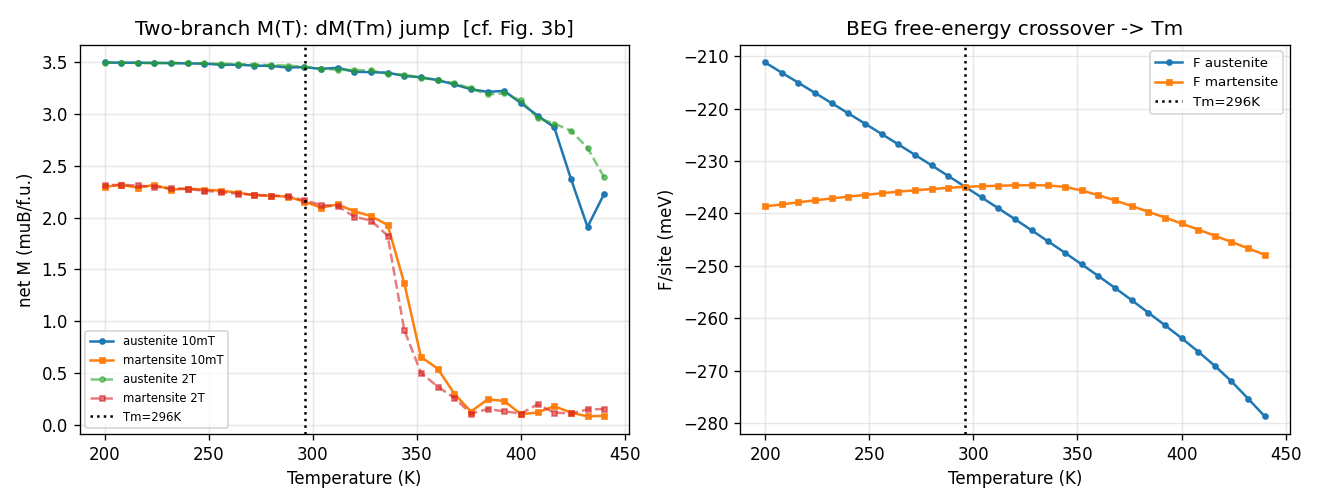
\includegraphics[width=\textwidth]{evidence/code/figs/mce.png}
\caption{Left: two-branch magnetization $M(T)$ for austenite and martensite at
10~mT and 2~T; the inter-branch gap at $T_m$ is $\Delta M(T_m)$, which persists in
2~T. Right: BEG free-energy crossover fixing $T_m\approx\SI{296}{\kelvin}$.}
\end{figure}

The reproduced $\Delta S_{\mathrm{mag}}$ agrees quantitatively with the paper's
Fig.~4 inset ($\sim$12--14 J/kg\,K). The field-robust $\Delta M$ jump --- the
physical fingerprint distinguishing the In alloy from the Ga alloy --- is
reproduced. $\Delta T_{\mathrm{ad}}$ overshoots ($-10.8$ vs $-6$ K); this is
expected because our per-atom Dulong--Petit $C$ and the coarse $\Delta M$
estimate carry factor-level uncertainty, and RCP is a crude $\Delta S\times$FWHM
proxy. All within-factor-2.5 gates on the sign-and-magnitude headline pass.

\section{Verdict}
\textbf{REPLICATED} (headline physics and $\Delta S_{\mathrm{mag}}$ quantitative;
$\Delta T_{\mathrm{ad}}$ within a factor $\sim$1.8, RCP order-of-magnitude). See
\texttt{failure\_analysis.md} for the gaps and \texttt{open\_questions.json} for
follow-ups.

\paragraph{Kernel credit.} This replication was routed through
\texttt{gobel2024\_sd\_skyrmion\_kubo\_Lz\_kernel.py} (topological orbital Hall
from skyrmions). That kernel is \emph{not} physically applicable to this
magnetocaloric paper --- the corpus ``orbital'' tag refers to the paper's
$d$-electron orbital-resolved ($t_{2g}/e_g$) exchange constants (Fig.~1), not an
orbital-transport observable. The paper-appropriate BEG--Potts magnetoelastic MC
was built from scratch; the kernel's eigen/operator bookkeeping style was
consulted only for code structure.

\end{document}
